\section{Measurement Details and Additional Diagnostics}
\label{appendix:gd-raw-alignment}

\subsection{Objectives and Measurement}

The tanh MLP has two 200-unit hidden layers and minimizes half-squared
error summed over ten output coordinates and averaged over the first
5,000 training images. ResNet-32 minimizes mean cross-entropy on all
50,000 training images. The word-level Transformer has two layers,
two attention heads, and embedding/feed-forward dimensions of 200;
its objective is token-weighted negative log-likelihood. In the GD
comparison, constant learning rates share frozen seed-0 initial tensors
within each case. GD uses no momentum, decay, clipping, augmentation,
dropout or schedule.

The MLP uses coordinate-wise standardization and ResNet uses channel-wise
standardization, both based on the complete CIFAR-10 training split.
ResNet's objective averages the same 50 fixed groups of 1,000 images,
with batch normalization performed separately within each group.
Accumulating all group gradients gives the gradient of this fixed
objective; physical batching introduces no random sampling.

For the Transformer, the corpus is arranged into 20 fixed streams and
causal chunks of at most 35 tokens. Eight stream-tail tokens and the
20 initial context tokens have no training target; short chunks retain
their valid targets, and padding is excluded from the loss. The resulting
59,680 sequences contain 2,088,600 training targets. The 33,278-word
vocabulary follows the first-occurrence dictionary over training,
validation and test text in the PyTorch word-language-model example,
revision \texttt{13acec6d7c78}~\cite{pytorchWordLanguageModelPinned}.
The same pinned example supplies the Transformer implementation.
All reported comparisons concern training-objective dynamics.

Physical accumulation uses 1,000-image chunks for the MLP, the fixed
1,000-image groups for ResNet, and 64-sequence chunks for the Transformer.
The complete objective is accumulated before each parameter update.
Training parameters and gradients are FP32, TF32 is disabled, and
diagnostic reductions are FP64. The nine conditions give paired
learning-rate comparisons within three model cases. Architectures,
objectives and data coverage differ between cases, and each case has
one initialization. The computational cost stated in
Section~\ref{subsec:normalized-displacement} is algorithmic; measured
runtime overhead depends on implementation and is left to a separate
benchmark.

Cosines with zero norms and the first unpaired gradient are undefined.
Complete 50-observation trailing means summarize the GD diagnostic curves;
pointwise quantities are computed before averaging. Endpoint losses and
$R_{3000}$ are unsmoothed.

\subsection{Unsmoothed Alignment and Temporal Accounting}

Figure~\ref{fig:gd-raw-alignment} supplies the unsmoothed consecutive
cosines underlying Fig.~\ref{fig:gd-alignment-displacement}(a)--(c).
Complete trailing means suppress short transients and shift the displayed
transition relative to the first negative pair. In particular, the MLP
at $\eta=0.04$ reverses near initialization and then returns to positive
alignment before its later negative phase. These raw traces distinguish transient regime changes from sustained
destructive phases.

\begin{figure*}[!t]
  \centering
  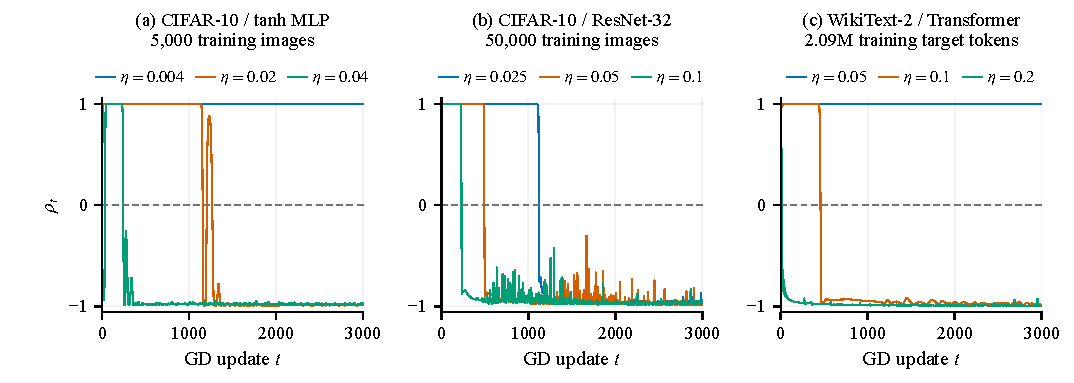
\includegraphics[width=\textwidth]{figures/analysis024/eos_gd_rho_3k.pdf}
  \caption{Unsmoothed consecutive-gradient cosine for the nine full-GD
  conditions in Section~\ref{sec:gd-experiments}, with 2,999 defined pairs
  per condition. Columns show (a) MLP, (b) ResNet-32 and (c) Transformer.
  The dashed horizontal reference is zero. Blue, orange and green identify
  increasing learning rates within each case, as given in the legends.
  Every curve uses seed 0 and covers the same 3,000-update horizon;
  the first undefined pair is omitted and there is no temporal or seed
  averaging. Coincident positive curves can overlap exactly.}
  \label{fig:gd-raw-alignment}
\end{figure*}

For the complete prefix of $T$ gradients, define the traveled distance
and the temporal contributions as
\begin{equation}
\begin{aligned}
 P_T&:=\eta\sum_{t=1}^{T}\|g_t\|,\\
 I_T^{(1)}&:=2\sum_{t=2}^{T}g_{t-1}^{\top}g_t,\\
 I_T^{(>1)}&:=2\sum_{\substack{1\leq u<t\leq T\\t-u>1}}g_u^{\top}g_t,\\
 I_T&:=I_T^{(1)}+I_T^{(>1)}
      =\Bigl\|\sum_{t=1}^{T}g_t\Bigr\|^2-\sum_{t=1}^{T}\|g_t\|^2.
\end{aligned}
\label{eq:gd-temporal-accounting}
\end{equation}
Table~\ref{tab:gd-temporal-accounting} reports these quantities at $T=3000$.
The interaction columns use raw gradients and include the factor of two;
they are not multiplied by $\eta^2$. The total is positive in all nine
conditions, whereas the adjacent contribution is negative in seven.
The positive total demonstrates longer-range reinforcement alongside
adjacent destruction. Magnitudes are compared within each model and
its fixed parameterization.


\subsection{Retrospective Loss Approximation}

For each gradient pair indexed by $t=2,\ldots,3000$, let
$\delta\mathcal L_{t-1}:=\mathcal L(\theta_{t-1})-\mathcal L(\theta_{t-2})$.
We compare this observed change with the gradient-based approximation
\begin{equation}
  \widehat{\delta\mathcal L}_{t-1}
  :=-\frac{\eta}{2}\|g_{t-1}\|^2
  \left(2-\eta\widehat\kappa_t\right).
  \label{eq:gd-loss-surrogate}
\end{equation}
The normalized absolute discrepancy is
\begin{equation}
 e_t:=\frac{|\delta\mathcal L_{t-1}-\widehat{\delta\mathcal L}_{t-1}|}
                 {\eta\|g_{t-1}\|^2}.
 \label{eq:gd-loss-audit-residual}
\end{equation}
The denominator is the magnitude of the first-order full-GD descent term.
It is nonzero for every measured pair. Table~\ref{tab:gd-loss-audit}
reports the median over all 2,999 pairs and the count of opposite signs.
The final update is excluded because its subsequent gradient was not
recorded. All inputs are unsmoothed; the table uses no seed aggregation.

For the threshold sensitivity columns, define
\begin{equation}
 h_t(\tau):=\tau\max\{ |\mathcal L(\theta_{t-2})|,
                         |\mathcal L(\theta_{t-1})|\}.
\end{equation}
A transition is eligible only when both
$|\delta\mathcal L_{t-1}|>h_t(\tau)$ and
$|\widehat{\delta\mathcal L}_{t-1}|>h_t(\tau)$.
Each cell prints opposite-sign transitions divided by its eligible count;
the median discrepancy uses all pairs. The thresholds provide a descriptive
sensitivity analysis. The comparison uses the subsequent gradient and
repeated transitions within one trajectory; finite-step, nonsmooth
and numerical effects all contribute to the discrepancy.
For the highest-rate Transformer, the unthresholded signs disagree in
$44.2\%$ of transitions; excluding changes below the $10^{-5}$ relative
threshold leaves $43.7\%$ disagreement. Thus a projected change near two
identifies the oscillatory regime at the scale shown in the main
figures, while stepwise loss signs remain sensitive to nonlinear effects.


\subsection{Backward-Lag Measurements}

The backward profiles use the largest GD rate in each model, with exact
full-objective gradients from separately recomputed 256-update
continuations. Retained states 500, 2000 and 3000 supply common starting
parameters; their endpoints are states 756, 2256 and 3256 (gradient
indices 757, 2257 and 3257). Figure~\ref{fig:gd-backward} uses the middle
endpoint in every model, providing a common trained-state comparison.
Each curve holds that
endpoint fixed, includes every lag through 256, and uses no temporal
averaging or compression. FP64 products of FP32 vectors were checked
independently on CPU and GPU; selected retained vectors supply additional
local checks. Later floating-point trajectories can depart from earlier
replays despite identical starting tensors, so these profiles are
separate continuations, not reconstructed pairs from Figs.~\ref{fig:gd-loss}
and~\ref{fig:gd-alignment-displacement}. At all nine measured endpoints,
both positive and negative similarities occur within lags 193--256;
their amplitudes vary substantially across endpoints.

\subsection{Mini-Batch Comparison}

The mini-batch comparison uses three initializations for each objective.
The MLP reuses the completed 5,000-image experiment at $\eta=0.02$,
with batches $32,128,512,2048,5000$. Fresh 2,000-update GD references
at $\eta=0.1$ and $0.2$ supply ResNet and Transformer starting states.
ResNet samples $1,5,20$ or all $50$ fixed 1,000-image normalization
groups, preserving each image's normalization context; its figure axis
reports image counts. Transformer batches contain $8,32,128,512$ or all
$59{,}680$ prepared sequences, with $M=2{,}088{,}600$ supervised tokens
in the complete training objective. If $\ell_i$ is sequence $i$'s summed
token loss, the sampled estimator is
$\frac{N}{bM}\sum_{i\in B}\ell_i$, with $N=59{,}680$; a random sampled-token
denominator would change this estimator. Every stochastic batch is a
uniform subset without replacement, independently redrawn at each update.
Batch sizes share prefixes of a common permutation within a repetition;
permutations are independent across updates and repetitions. Parameters
and gradients use FP32, reductions use FP64, and TF32 is disabled.
Full-loss evaluations cover every training image or supervised token.
Cosines average all
199 defined consecutive pairs; retention uses all 200 applied gradients.
Eight repetitions are averaged within initialization before the three
initializations receive equal weight. The plotted range represents variation
among initialization-block means. Cases differ in objective, architecture,
data size and selected learning rate; the controlled contrasts are
within each case.

Cloud runs use PyTorch 2.8/CUDA 12.8. The Transformer uses RTX5090 and
512-sequence physical accumulation, without changing effective batches.
ResNet uses L40S/RTX4090; seed~2's smallest two batches use GB10/PyTorch
2.11/CUDA 13 from hash-identical cloud checkpoints. Complete-gradient and
short replay checks qualify this runtime; a 200-update initial full-GD bridge
has endpoint parameter relative error $2.36\times10^{-7}$ versus the cloud.
Batch and runtime effects are confounded in this block; shading includes
initialization and runtime variation, and long trajectories can drift
beyond the short replay agreement. Initial full controls for ResNet seed~2 and Transformer seed~0
reuse the exact first 200 reference updates, with separate endpoint losses;
other controls execute independently. Audits of actual increments and endpoint
displacement quantify FP32 update roundoff.

\subsection{Spectral Context}

We measure the largest algebraic Hessian eigenvalue at states
$0,100,\ldots,3000$ using matrix-free Hessian--vector products and a
checked relative eigenpair residual of at most $0.005$. The Hessian
objective covers all 5,000 MLP training examples, but only the first
five fixed ResNet groups and the first 2,500 Transformer sequences.
Subset measurements follow the computational motivation
of~\cite{cohen2021edge} and describe sharpness on those fixed subsets. Reused MLP trajectories requested two largest eigenvalues
and the other runs requested one; we compare only the largest value.
Table~\ref{tab:gd-spectral-context} retains all nine final measurements.

Maximum pointwise eigenvalue concerns the most curved local direction,
whereas $\widehat\kappa_t$ concerns realized gradient change across a step.
Objective coverage and a finite-step Taylor remainder also affect their
comparison. Final spectral values and the late means in
Table~\ref{tab:gd-endpoints} use different temporal reductions. Both coverage and timing must therefore be matched for an
estimator-accuracy comparison. A state-matched local comparison would pair
the Hessian at state $s$ with the expansion for gradient index $t=s+2$;
the spectrum at state 3000 has no matching recorded gradient pair.



\begin{table*}[!t]
  \centering
  \caption{Complete-prefix temporal accounting at $T=3000$, with the
  quantities defined in Eq.~\eqref{eq:gd-temporal-accounting}.
  $P_{3000}$ is path length; the last three columns are raw-gradient
  interactions. All nine conditions use one shared initialization per case.
  Values are rounded only for display, so displayed components may not
  sum exactly to the displayed total.}
  \label{tab:gd-temporal-accounting}
  \small
  % Generated by Analysis024/08_build_manuscript_assets.py; do not edit numbers.
\begin{tabular}{@{}llrrrr@{}}
\toprule
Model & $\eta$ & $P_{3000}$ & $I_{3000}^{(1)}$ & $I_{3000}^{(>1)}$ & $I_{3000}$ \\
\midrule
MLP & 0.004 & 1.1976 & $1.270\!\times\!10^{2}$ & $5.634\!\times\!10^{4}$ & $5.647\!\times\!10^{4}$ \\
MLP & 0.02 & 64.3608 & $-1.217\!\times\!10^{4}$ & $3.063\!\times\!10^{4}$ & $1.846\!\times\!10^{4}$ \\
MLP & 0.04 & 185.5420 & $-1.662\!\times\!10^{4}$ & $2.225\!\times\!10^{4}$ & $5.630\!\times\!10^{3}$ \\
\midrule
ResNet-32 & 0.025 & 41.1785 & $-2.528\!\times\!10^{3}$ & $5.325\!\times\!10^{4}$ & $5.072\!\times\!10^{4}$ \\
ResNet-32 & 0.05 & 146.3482 & $-7.380\!\times\!10^{3}$ & $3.603\!\times\!10^{4}$ & $2.865\!\times\!10^{4}$ \\
ResNet-32 & 0.1 & 372.7896 & $-1.076\!\times\!10^{4}$ & $2.451\!\times\!10^{4}$ & $1.375\!\times\!10^{4}$ \\
\midrule
Transformer & 0.05 & 15.6687 & $1.629\!\times\!10^{2}$ & $5.100\!\times\!10^{4}$ & $5.116\!\times\!10^{4}$ \\
Transformer & 0.1 & 111.8465 & $-7.767\!\times\!10^{2}$ & $2.464\!\times\!10^{4}$ & $2.387\!\times\!10^{4}$ \\
Transformer & 0.2 & 405.8404 & $-2.682\!\times\!10^{3}$ & $1.336\!\times\!10^{4}$ & $1.067\!\times\!10^{4}$ \\
\bottomrule
\end{tabular}

\end{table*}

\begin{table*}[!t]
  \centering
  \caption{Retrospective check of the local loss approximation for all nine
  conditions. The unthresholded count and median $e_t$ use 2,999 transitions
  per condition. Each threshold cell gives opposite signs / eligible
  transitions; eligibility requires both change magnitudes to exceed
  $h_t(\tau)$. These descriptive temporal counts are not independent-sample
  predictive accuracies.}
  \label{tab:gd-loss-audit}
  \small
  % Generated by Analysis024/08_build_manuscript_assets.py; do not edit numbers.
\begin{tabular}{@{}llrrrrr@{}}
\toprule
 & & & & \multicolumn{3}{c}{Opposite signs / eligible transitions at threshold $\tau$} \\
\cmidrule(l){5-7}
Model & $\eta$ & No threshold & Median $e_t$ & $10^{-7}$ & $10^{-6}$ & $10^{-5}$ \\
\midrule
MLP & 0.004 & 0/2999 & $2.905\!\times\!10^{-4}$ & 0/2999 & 0/2999 & 0/2999 \\
MLP & 0.02 & 145/2999 & $6.146\!\times\!10^{-4}$ & 145/2998 & 145/2998 & 141/2989 \\
MLP & 0.04 & 281/2999 & $7.343\!\times\!10^{-3}$ & 281/2999 & 281/2998 & 280/2994 \\
\midrule
ResNet-32 & 0.025 & 595/2999 & $1.030\!\times\!10^{-2}$ & 595/2999 & 592/2991 & 570/2934 \\
ResNet-32 & 0.05 & 694/2999 & $2.347\!\times\!10^{-2}$ & 694/2999 & 692/2997 & 682/2978 \\
ResNet-32 & 0.1 & 814/2999 & $2.324\!\times\!10^{-2}$ & 813/2997 & 813/2997 & 809/2989 \\
\midrule
Transformer & 0.05 & 0/2999 & $2.381\!\times\!10^{-5}$ & 0/2999 & 0/2999 & 0/2999 \\
Transformer & 0.1 & 542/2999 & $1.398\!\times\!10^{-2}$ & 541/2997 & 534/2977 & 436/2703 \\
Transformer & 0.2 & 1325/2999 & $6.323\!\times\!10^{-2}$ & 1324/2996 & 1319/2989 & 1239/2837 \\
\bottomrule
\end{tabular}

\end{table*}

\begin{table*}[!t]
  \centering
  \caption{Final spectral context at parameter state 3000. Only the MLP
  measurement covers its complete training objective. ResNet and Transformer
  use fixed subsets of the stated size; residual-checked eigenpairs do not
  establish subset representativeness. All conditions use seed 0.}
  \label{tab:gd-spectral-context}
  \small
  % Generated by Analysis024/08_build_manuscript_assets.py; do not edit numbers.
\begin{tabular}{@{}lllr@{}}
\toprule
Model & $\eta$ & Hessian objective coverage & $\eta\lambda_{\max,3000}$ \\
\midrule
MLP & 0.004 & Full 5,000 images & 0.3168 \\
MLP & 0.02 & Full 5,000 images & 2.2157 \\
MLP & 0.04 & Full 5,000 images & 2.3259 \\
\midrule
ResNet-32 & 0.025 & Fixed 5,000-image subset & 2.8176 \\
ResNet-32 & 0.05 & Fixed 5,000-image subset & 2.6599 \\
ResNet-32 & 0.1 & Fixed 5,000-image subset & 3.2488 \\
\midrule
Transformer & 0.05 & Fixed 2,500-sequence subset & 1.7229 \\
Transformer & 0.1 & Fixed 2,500-sequence subset & 2.2752 \\
Transformer & 0.2 & Fixed 2,500-sequence subset & 3.1202 \\
\bottomrule
\end{tabular}

\end{table*}


\subsection{Controlled Adam Measurements and Spike Analysis}
\label{appendix:adam-measurements}

Adam uses the complete objectives and frozen initial tensors specified
above. All trainable parameters enter the diagnostics; parameters,
gradients and moments are FP32, reductions are FP64, and TF32 is disabled.
All MLP rates use one RTX 5070 Ti. In increasing-rate order, ResNet uses
PRO 4000, a PRO 6000 partition and RTX 4090; Transformer uses RTX 4090,
PRO 4500 SE and RTX 4090. Initial-gradient agreement is verified across
workers. Hardware variation and later finite-precision drift accompany
the rate comparison. Held-out splits are evaluated every 128 updates;
rate selection uses training calibration.

At state $\theta_s$, the raw gradient is $g_{s+1}$ and the first moment
$m_{s+1}$ includes that gradient before update $s+1$. This is the clock
used in the Adam figures. Momentum cosines replace $g$ by $m$ in
Eq.~\eqref{eq:rho}. Relative norms use the first displayed state, as
specified in Fig.~\ref{fig:adam-spikes}; event statistics use the fixed
pre-rise baseline. All losses and micro-plots are unsmoothed.
Initial adjacent diagnostics and zero-denominator ratios are undefined.
The terminal raw-gradient diagnostic is recorded after update 1,024
without applying another update.

Event extraction searches every loss state from initialization,
using strict increases and the first return in
Eq.~\eqref{eq:adam-spike-boundaries}. The density includes all 806
recovered excursions. The anatomy sample keeps 129 with increase
$>10\%$ and observed recovery; two above-threshold events without
recovery by update 1,024 are excluded. Two initialization events
lack pre-rise cosine and projected change, leaving 127 scatter points.
Each event receives equal weight; recovery summaries first average
within the event. Standard deviations use denominator $n-1$.

The seven scatter fits use ordinary least squares with an intercept,
separate coefficients per model/rate, and
$\log_{10}(\mathcal L_{p_i}/\mathcal L_{a_i})$ as response.
Reported $R^2$ uses that response in the fitting sample; dashed extensions
are extrapolations. Densities use Gaussian kernels on log percentage
increase. The common bandwidth within a model is the pooled sample
standard deviation times pooled $n^{-1/5}$, and each rate's density
has unit mass in those coordinates. These exploratory event summaries
describe repeated observations within one initialization per model.
Analysis036 retains source hashes, segmentation checks and scalar histories.
